\section{Project organisation and means implemented}
\label{sec:org}

\subsection{Scientific coordinator and its team}

\Comments{
  In the case of a Young Researchers Project (JCJC), 
Present the scientific coordinator and his/her role in the project, present his/her position within the organisation of the host laboratory 
Present the scientific coordinator’s team, its quality and complementarity
}

%------------------------ team
\textbf{Tristan Roussillon} (33 years old) is the principal investigator (PI) of the project
and will work on all tasks. Implication: \textbf{30} person months (PM). 
He completed his PhD in 2009 and since 2012, he is Associate Professor of Computer Science at INSA Lyon
and a member of LIRIS. 
He has coauthored a book chapter on digital geometric estimators \cite{Coeurjolly2012} and
has recently obtained several results on normal vector computation \cite{LPRTCS2016,LPRDGCI2016,LPRJMIV2017}.    
He has written a total of 8 papers in peer-reviewed international journals (PR, CVIU, JMIV, DAM, \ldots) 
and 14 in conferences (DGCI, ICPR,\ldots).

The project will also involve specialists in digital geometry and combinatorics on words. 
\begin{table}[h]
\small
\centering
\begin{tabular}{|cccl|}
\hline
Collaborator & Position & Lab & Expertise \\ \hline
\hline
\textbf{D. Coeurjolly} & DR & LIRIS & digital and comput. geometry, geometry processing \\ \hline
\textbf{B. Kerautret} & MdC & LORIA & digital geometry, image analysis \\ \hline
\textbf{S. Labb\'{e}} & CR & LABRI & multidim. cont. frac. alg., combinatorics on words \\ \hline
\textbf{J-O. Lachaud} & Pr & LAMA & digital geometry and topology, image analysis \\ \hline
\hline
\end{tabular}
\normalsize
\end{table}
%% \begin{table}[h]
%% \small
%% \centering
%% \begin{tabular}{|ccclcc|}
%% \hline
%% Collaborator & Position & Lab & Expertise & WP & PM \\ \hline
%% \hline
%% \textbf{D. Coeurjolly} & DR & LIRIS & digital and comput. geometry, geometry processing & 2-3 & 5 \\ \hline
%% \textbf{B. Kerautret} & MdC & LORIA & digital geometry, image analysis & 3 & 12 \\ \hline
%% \textbf{S. Labb\'{e}} & CR & LABRI & multidim. cont. frac. alg., combinatorics on words & 0-1 & 12 \\ \hline
%% \textbf{J-O. Lachaud} & Pr & LAMA & digital geometry and topology, image analysis & 0,2-3 & 6 \\ \hline
%% \hline
%% \end{tabular}
%% \normalsize
%% \end{table}

TODO qqs phrases de presentations pour chacun ?
\textbf{D. Coeurjolly} 
\textbf{B. Kerautret} 
\textbf{S. Labb\'{e}} 
\textbf{J-O. Lachaud}

%TODO research highlights en citant des contributions dans le domaine. 

This team gathers all the expertise required to ensure the success of the project.
Furthermore, this project will let the team members maintaining their lead in digital surface analysis 
and more generally in digital geometry and combinatorics on words for digital imagery. 


%% \subsection{Means of achieving the objectives}

%% In this section, we first detail and justify the scientific programme with regard to the project objectives.
%% We then describe the requested means. 

\subsection{Scientific program}
\label{sec:wp}

\Comments{Set out the scientific programme and justify the work programme's task breakdown with regard to the objectives being pursued.
For each task, describe the objectives, the work programme, deliverables, partners' contributions, methods and technical decisions, risks, and fall-back solutions. 
Illustrate the programme with a Gantt chart. 
}

This \textbf{four-year project} will be divided into four work packages (WP).
The two first corresponds to goal G1, whereas the two last correspond
respectively to goals G2 and G3 (see \sect{sec:goals} for the goal description).
We have decided to have two WPs for G1 because this goal has two distinct sides,
each requiring distinct expertise. On one hand, we want to improve various
features of plane-probing algorithms, even in the planar case. Due to
preliminary works, we have in mind many short-term tasks for this.
On the other hand, we want to associate to the state of a plane-probing
algorithm a piece of digital plane that fits to the digital surface in order
to correctly process non-planar parts. This requires not only expertise
in digital geometry but also in multidimensional continued
fractions algorithms and combinatorics on words (see \sect{sec:dps} and below).

\subsubsection{WP0: Plane-probing algorithms}
\label{wpPPA}

%% \WP{Find the ultimate plane-probing algorithm (part of G1)}
%%    {S. Labb\'{e}, J-O. Lachaud, \textbf{T. Roussillon}}
%% \medskip

As explained in \sect{sec:dps}, a plane-probing algorithms sparsely probes the data points
around a starting point to compute a local normal direction. Several algorithms of this kind
has been proposed by the principal investigator and its collaborators
\cite{LPRTCS2016, LPRDGCI2016, LPRJMIV2017}.
What makes them original in regard to the state of the art, is that they decide on-the-fly
how to probe the digital surface, without any parameter or any prior order.

The last proposed algorithm, called \emph{R-algorithm} in \cite{LPRJMIV2017}, is the most
local algorithm. In order to explain what we mean by \emph{local}, we recall that
the R-algorithm iteratively deforms an initial tetrahedron. One vertex, denoted by $q$,
is however fixed and is always projected into the opposite triangular facet, denoted by
$F := (v_0,v_1,v_2)$. For any permutation $\sigma$ over $\{0,1,2\}$, $F$ defines a 2D
lattice embedded in 3D:
$\Lambda := \{ v_{\sigma(0)} + k (v_{\sigma(1)}-v_{\sigma(0)}) + k' (v_{\sigma(2)}-v_{\sigma(1)}) \ | \ k,k' \in \Z \}$. 
The basis $(v_{\sigma(1)}-v_{\sigma(0)}, v_{\sigma(2)}-v_{\sigma(1)})$ is \emph{reduced} if and only
if they are the two shortest nonzero vectors of $\Lambda$. By extension $F$ is said reduced
if there exists a permutation $\sigma$ such that $(v_{\sigma(1)}-v_{\sigma(0)}, v_{\sigma(2)}-v_{\sigma(1)})$
is reduced. The following conjucture is experimentally true but not yet proved:

\begin{Conjecture}
  \label{conj:reduction}
  The facet $F$ returned by the R-algorithm is reduced at least every two steps and
  is always reduced at the last step.  
\end{Conjecture}

A first task of this WP is to prove this conjecture, because it may be
a key ingredient to certify the locality of the R-algorithm and answer
the following questions: can we bound by above the distance of the probed
points to the starting point? 
what is the minimal part $\Part \subset \Plane{\mu}{\vec{n}}$ for which the
R-algorithm returns the normal $\vec{n}$ when applied to $\Part$?
can we characterize the behavior of the R-algorithm on a convex or arbitrary
part of a digital surface?

\begin{Task}
  \label{task:reduction}
  Prove conjecture~\ref{conj:reduction} and certify the locality of the R-algorithm. 
\end{Task}

Another task in this WP is related to the starting point. In \cite{LPRJMIV2017},
it must be a \emph{reentrant corner}. This restriction avoids degenerate cases, but
limit the pratical usage of the algorithm for digital surface analysis
(see fig.~\ref{fig:snow}). Raising this restriction to points whose neighboring
surfels form a flat part along one or two axis is however just a technical
problem that can be quickly solved. A more important challenge is that the R-algorithm
stops prematurately and outputs only an approximation of the normal vector for some
well-indentified starting points, which are not located deeply enough in the digital
surface. Even if we know how to detect and remove approximated results
\emph{a posteriori} \cite{LPRJMIV2017}, it would be quite interesting to translate
the starting point to deeper and deeper positions in order to avoid producing any
approximated results.
%TODO ne remet pas en cause la localite.
%Finally, it remains the \emph{sailent corners}. 
%how to retrieve complementary facets ?
TODO: parler des facettes complementaires ?

\begin{Task}
  \label{task:start}
  Modify the R-algorithm so that it can be run from any starting point. 
\end{Task}


\Risks
Preliminary works have considerably reduced the risks in this WP. Task~\ref{task:start}
can be done within one year. If we face to a difficulty that cannot be overcomed,
we will resort to the R-algorithm as it is described in \cite{LPRJMIV2017} and use it
to improve the approach of \citeauthor*{Charrier2011} \cite{Charrier2011}, as explained
in \sect{sec:methodo}. Task~\ref{task:reduction} is very important to rely on provable
properties but not completing it does not prevent us from developing practical algorithms.

\Success
\begin{itemize}
    \item A plane-probing algorithm, which always leads to a
      reduced facet of normal $\vec{n}$ when applied to a digital
      plane $\Plane{\mu}{\vec{n}}$ from any starting points.
    \item Implementation of the algorithm in \DGtal.   
    \item Theoretical guarantees about the locality of the algorithm
      for convex digital surfaces.  
\end{itemize}

\Members{S. Labb\'{e}, J-O. Lachaud, \textbf{T. Roussillon}}
  
\subsubsection{WP1: Pattern generation}
\label{wpPattern}

%% \WP{Generate a pattern under shape constraints (part of G1)}
%%    {S. Labb\'{e}, \textbf{T. Roussillon}}
%% \medskip

Plane-probing algorithms probe for data points in a sparse way.
This is perfect for digital plane recognition, but not for pieces
of digital plane on digital surfaces. Evolving tetrahedra may jump
over holes or cracks in the surface for instance. Therefore,
we have to associate a piece of digital plane
to the current facet and check whether it fits to the digital surface
or not.

Instead of digitizing the current facet, we choose to generate a piece
of digital plane closely related to the matrix sequence computed by
the plane-probing algorithms (see \sect{sec:dps}). We believe that
this approach will not only provide a hierarchy of pieces of digital
plane with controlled shape, but also a deep understanding of the
combinatorial structure of digital planes. If this combinatorial
structure is completely understood, it will be possible to implicitely
describe various pieces of digital plane by exchanging some well-identified
parts of it, which will lead to a more flexible algorithm. 

The challenge in this WP is to generate digital plane segments (DPSs)
having several properties \cite{Jamet2016}:
\begin{enumerate}
\item[(P1)] they must be included in the tangent digital plane;
\item[(P2)] at least two independent period vectors should be deduced from them
  so that the whole tangent digital plane is implicitly described by translation
  (and that is why such DPSs are called \emph{patterns});
\item[(P3)] they should form a connected set;
\item[(P4)] they should be as small as possible to avoid redundancy,
  \eg $n_i$ surfels of normal vector $\vec{e}_i$, where $n_i$ is the i-th coordinate
  of $\vec{n}$. 
\end{enumerate}
We can add other properties about their shape: symmetry to their central part \cite{Labbe2015},
convexity, smallest possible elongation or maximal distance to the starting point.
%% It may also contain the standard digitization of the current facet returned by
%% a plane-probing algorithm. 

As reported in \sect{sec:dps}, there are two main generic methods for generating patterns
from an arbitrary multidimensional continued fractions (MCF) algorithm:
\begin{itemize}
\item[(M1)] the first one is based on dual substitutions, 
\item[(M2)] the second one is based on a translation-union algorithm.
\end{itemize}
We believe that these two approaches are closely related, but this requires
further investigation because they rely on different frameworks. 
%TODO lien avec Christoffel graph


\begin{Task}
  \label{task:genmeth}
  Study methods M1 and M2 on arbitrary MCF algorithms and compare them.   
\end{Task}

Even if MCF algorithms usually guarantee some of the above properties (at least P1 and P2),
they do not take into account the pattern shape. As any other MCF algorithm, the R-algorithm
also produces a sequence of matrices, denoted by $M_1..M_n$. We believe that the R-algorithm
is a good candidate for methods M1 and M2 in order to generate patterns with shape
constraints because it returns a reduced triangular facet.

One difficulty is that several substitutions can be associated to the same matrix
(but a substitution has one incidence matrix). First, we may consider all the possible
substitution sequences
$\Sigma := \{ \sigma_1..\sigma_n \ | \ \sigma_i \text{ is a possible substitution for } M_i \}$.

\begin{Task}
  \label{task:genexp}
  Experimentally check if the properties P1-P4 hold for patterns generated from $\Sigma$
  by methods M1 and M2.  
\end{Task}

Although it is hardly never investigated in the field of MCF algorithms, the choice of a
substitution can play an important role, especially for P3 and P4. In our geometric setting,
we can expect a criterion for choosing a convenient substitution at each step. 

\begin{Task}
  \label{task:genpat}
  Generate a pattern having at least properties P1-P4 in the course of the R-algorithm. 
\end{Task}

For this WP, we expect strong and rich interactions between digital geometry, combinatorics on words
and the field of MCF algorithms as highlighted by the collaborators' expertise.

\Risks
We do not know if it is possible to generate patterns with all the above properties
or an appropriate subset of them in order to correctly process non-convex parts,
in spite of promising results (TODO fig). Still, we have algorithmic solutions
\cite{LPRJMIV2017} to cope with these problems, which alleviate such risk. 
On the contrary, a success in this WP would lead to both theoretical results
on MCF algorithms and related geometric problems, and a speed-up in the analysis
of digital surfaces thanks to arithmetic and combinatorial properties.  

\Success
\begin{itemize}
  \item A pattern generation algorithm based on the R-algorithm (or another plane-probing algorithm).
  \item Implementation of the algorithm in \DGtal.
  \item Theoretical guarantees about the shape of the generated pattern. 
\end{itemize}

\Members{S. Labb\'{e}, \textbf{T. Roussillon}}

\subsubsection{WP2: Geometric inference and applications}
\label{wpEstim}

%%   \WP{Propose a parameter-free, multigrid-convergent normal estimator (G2)}
%%    {C. Coeurjolly, J-O. Lachaud, \textbf{T. Roussillon}}
%% \medskip

 Most of the time, when we are working with a digital surface, we are 
interested in the geometry of a continuous shape whose digitization is the input digital data.
We expect that a given geometric quantity, such as a normal vector, computed at a point of a digital surface
is close to the one of the underlying continuous shape at a close enough point. 
This WP aims at providing efficient, parameter-free and multigrid-convergent estimators based of
the output of plane-probing algorithms: normal vector (and surfel area as a by-product),
distance to boundary, voxel coverage (fig.~\ref{fig:2D}).

\begin{Task}
  \label{task:normal}
  Propose a parameter-free normal estimator based on plane-probing algorithms and
  derive other first-order estimators.  
\end{Task}

The accuracy of a multigrid-convergent estimator depends on the resolution: the higher the resolution,
the more accurate the estimator. We will experimentally and theoretically study the estimation accuracy
for shapes digitized at increasing resolutions. 

\begin{Task}
  \label{task:conv}
  Study the estimation accuracy of the proposed estimators for smooth shapes digitized at increasing resolutions. 
\end{Task}

Plane-probing algorithms not only provide a normal vector but also position information,
which may be useful for many applications in graphics such as polyhedral approximation,
 or digital surface visualization. The goal of this WP is also to investigate at least
one of these applications.   


We can approximate a digital surface either by a polyhedral surface whose vertices 
are a subset of the input data points, as in convex hulls or relative convex hulls
\cite{Klette2001,Schultz2009} 
or a quadrangular mesh whose vertices are set to optimized positions so that it is
as smooth as possible. In the former problem, the facets returned by the
plane-probing algorithms will play an important role, while in the latter,
normal estimates are usually a key input of the optimization step (see for instance
\cite{Coeurjolly2017}).  

\begin{Task}
  \label{task:approx}
  Design an algorithm that computes a fair approximation of a digital surface. 
\end{Task}

Even if meshes can be efficiently visualized because of hardware support,
it may be interesting to directly render the input data. Ray casting can be used to
visualize digital surfaces. Results will be greatly improved by accurate normal estimates,
but also by accurate position estimates. In addition, voxel coverage and absorption can
also be used to remove staircase effects near shape borders in the resulting 2D view.

\begin{Task}
  \label{task:rendering}
  Design an algorithm that directly renders digital surfaces using first-order estimations.  
\end{Task}

\Risks
The main risk in this WP is that normal estimators
directly derived from plane-probing algorithms do not have the multigrid-convergence
property. In that case, fall-back solutions presented in \sect{sec:methodo} will achieve
multigrid-convergence without any parameter but at the price of a higher computational
cost and a lower accuracy in the localization of sharp features. 

\Success
\begin{itemize}
  \item A parameter-free and multigrid-convergent normal estimator.
  \item Implementation of the estimator in \DGtal.
  \item At least one of the tasks~\ref{task:approx} and \ref{task:rendering} is completed. 
\end{itemize}

\Members{C. Coeurjolly, J-O. Lachaud, \textbf{T. Roussillon}}
  
\subsubsection{WP3: Multiscale analysis}
\label{wpScale}

%% \WP{Develop a tool for a multiscale analysis of digital surfaces (G3)}
%%    {C. Coeurjolly, B. Kerautret, J-O. Lachaud, \textbf{T. Roussillon}}
%% \medskip

Digital surfaces may be degraded with \emph{noise}, especially in medical imaging.
Since noise usually affect only the finest levels of details, the following algorithm
is a way of coping with the problem: while there is noise, subsample by 2 the digital surface.
At the end, we get a noise-free digital surface, but at a potentially coarser level.
In addition, in case of non-uniform noise, the same applies only locally, \ie at each border voxel.  

The challenge here is to detect noise. This can be done by computing the growth rate of the
\emph{number} or \emph{size} of the computed facets for decreasing resolutions
%(see fig.~\ref{fig:snow} for an example of one such facet)
and by comparing it with the theoretical or experimental law for digitization of smooth shapes.
A significative difference between the two rates suggest that there is noise.
%TODO dire que dans cette partie, il y a des paramètres mais peu sensibles ?
This strategy has been used with success for digital curves \cite{Kerautret2012}
and the goal of this WP is to provide the theoretical results and tools required to apply it on digital surfaces. 

TODO illustration 2D ?

First, we will focus on the number of facets returned by plane-probing algorithms.
This global strategy, which provides a way of retrieving the scale with highest resolution
where noise is unlikely, is enough in case of uniform noise. 

\begin{Task}
  \label{task:global}
  Develop a tool that automatically returns the first noise-free subsample of an input 3D volume.
\end{Task}

Then, we will locally focus on the size of all facets covering a same data point for various resolutions. 

\begin{Task}
  \label{task:size}
  Define the size of a facet returned by plane-probing algorithms. Study the growth rate of the size
  for smooth parts at various resolution. 
\end{Task}

This local strategy, better than the previous one in case of non-uniform noise, provides however
a more complex output because a best scale is computed at each data point.
We can either simply output this information to feed other tools
or compute estimates during the scale detection, such as a normal estimator robust to noise.  

\begin{Task}
  \label{task:local}
  Develop a tool that automatically adds to a digital surface a scale value or
  a robust-to-noise normal estimate at each data point. 
\end{Task}
%alpha-shape, ball unions

\Risks
We are confident on the feasibility of the global strategy (task~\ref{task:global}),
because computed facets are closely related to convex hull facets in convex parts
and the growth rate of the number of convex hull facets is known for digitization
of convex smooth shapes \cite{Barany1998}. 
Task~\ref{task:local} could be however more difficult to complete
because it depends on a sound definition of the size of a facet (task~\ref{task:size})
for which the growth rate is clearly different for smooth parts on one hand
and noise or small-scale features on the other hand. If it is not the case, we can
resort to the length of the maximal DSSs along 2D slices as explained in \sect{sec:methodo}.

\Success
\begin{itemize}
  \item Implementation of the tools of tasks~\ref{task:global} and \ref{task:local}
    in \DGtalTools~ with companion papers in \IPOL.
\end{itemize}

\Members{C. Coeurjolly, B. Kerautret, J-O. Lachaud, \textbf{T. Roussillon}}

\subsection{Schedule and deliverables}
\label{sec:schedule}

TODO dependances des taches/WP et gantt ?
%WP sont ordonnes WP3 et WP2 graphe de dépendances des tâches ?
%1er WP en 1 an que du court terme
%les autres WP en 2 ans environ, 

\begin{figure}[htbp]
  \centering
  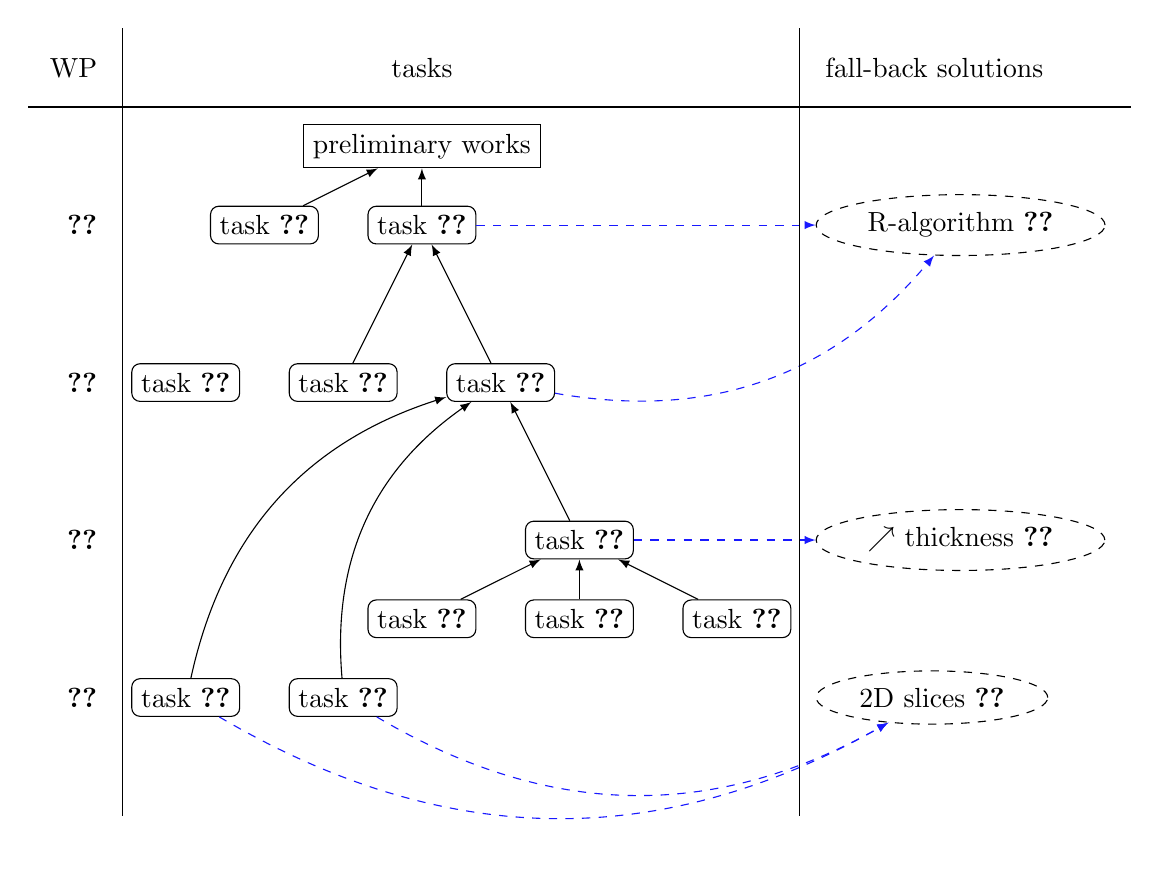
\begin{tikzpicture} 
\usetikzlibrary{shapes}

\tikzset{task/.style={draw,rectangle,rounded corners=3pt}}
\tikzset{sol/.style={draw,ellipse,dashed}}
\tikzset{toSol/.style={->,>=latex,dashed,color=blue!90!white}}
\tikzset{toTask/.style={->,>=latex}}

\node[left] at (0,8) {WP}; 
\node[left] at (0,6) {\ref{wp0}}; 
\node[left] at (0,4) {\ref{wp1}}; 
\node[left] at (0,2) {\ref{wp2}}; 
\node[left] at (0,0) {\ref{wp3}}; 

\node[right] at (9,8) {fall-back solutions};
\node[right,sol] (R) at (9,6) {R-algorithm \ref{riskppa}};
\node[right,sol] (C) at (9,2) { $\nearrow$ thickness \ref{riskestim}};
\node[right,sol] (S) at (9,0) {2D slices \ref{riskscale}};

\node at (4,8) {tasks};
\node[draw] (P) at (4,7) {preliminary works};

\node[task] (t0a) at (2,6) {task~\ref{task:reduction}};
\node[task] (t0b) at (4,6) {task~\ref{task:start}};
\draw[toTask] (t0a) -- (P);
\draw[toTask] (t0b) -- (P);
\draw[toSol] (t0b) -- (R);
\node[task] (t1a) at (1,4) {task~\ref{task:genmeth}};
\node[task] (t1b) at (3,4) {task~\ref{task:genexp}};
\node[task] (t1c) at (5,4) {task~\ref{task:genpat}};
\draw[toTask] (t1b) -- (t0b);
\draw[toTask] (t1c) -- (t0b);
\draw[toSol] (t1c) to[bend right] (R);
\node[task] (t2a) at (6,2) {task~\ref{task:normal}};
\node[task] (t2b) at (4,1) {task~\ref{task:conv}};
\node[task] (t2c) at (6,1) {task~\ref{task:approx}};
\node[task] (t2d) at (8,1) {task~\ref{task:rendering}};
\draw[toTask] (t2a) -- (t1c);
\draw[toSol] (t2a) -- (C);
\draw[toTask] (t2b) -- (t2a);
\draw[toTask] (t2c) -- (t2a);
\draw[toTask] (t2d) -- (t2a);
\node[task] (t3a) at (1,0) {task~\ref{task:global}};
\node[task] (t3b) at (3,0) {task~\ref{task:local}};
\draw[toTask] (t3a) to[bend left] (t1c);
\draw[toTask] (t3b) to[bend left] (t1c);
\draw[toSol] (t3a) to[bend right] (S);
\draw[toSol] (t3b) to[bend right] (S);

%\draw (-0.5,0) grid[step=1] (9,8);

\draw (-1,7.5) -- (13,7.5);
\draw (0.2,-1.5) -- (0.2,8.5);
\draw (8.8,-1.5) -- (8.8,8.5);

\end{tikzpicture}

  \caption{Tasks dependancy graph}
  \label{fig:tasks}
\end{figure}


\begin{figure}[htbp]
  \centering
  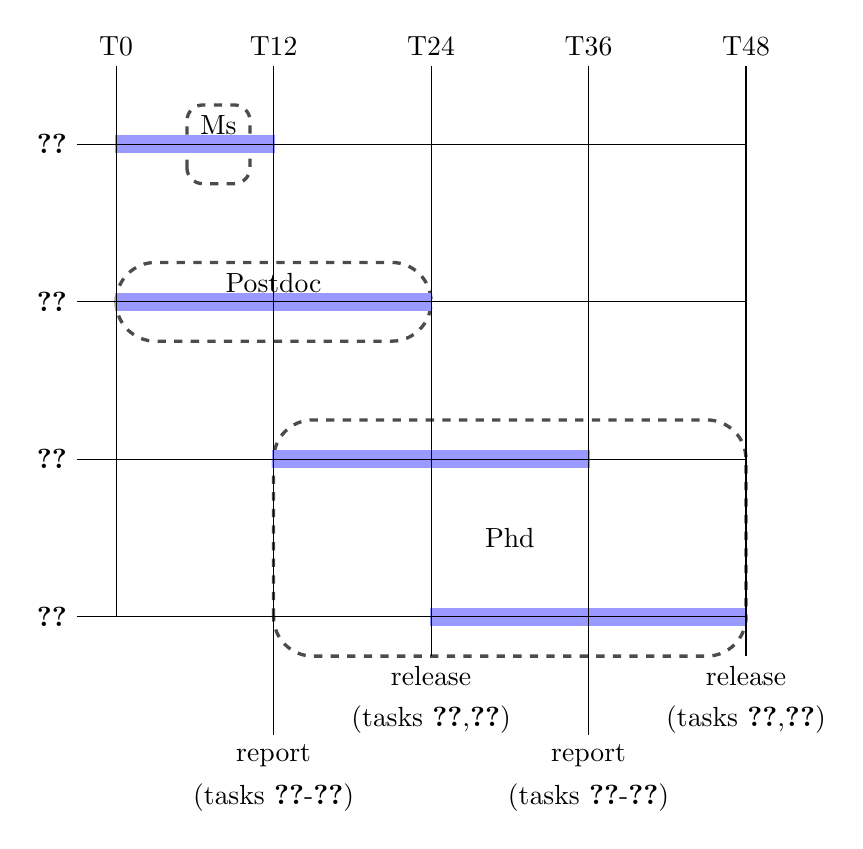
\begin{tikzpicture} 

\tikzset{%
  ebo unit/.store in=\ebounit,
  ebo corners/.style={rounded corners=#1\ebounit},
}

\node[above] at (0,7) {T0};
\node[above] at (2,7) {T12};
%\node[above] at (3,7) {T18};
\node[above] at (4,7) {T24};
\node[above] at (6,7) {T36};
\node[above] at (8,7) {T48};   

\node[left] at (-0.5,6) {\ref{wp0}}; 
\node[left] at (-0.5,4) {\ref{wp1}}; 
\node[left] at (-0.5,2) {\ref{wp2}}; 
\node[left] at (-0.5,0) {\ref{wp3}}; 

\tikzset{body/.style={very thick,dashed,color=black!70!white}}
\draw[draw,body,rounded corners=0.2cm] (0.9,5.5) rectangle (1.7,6.5) {};
\draw[draw,body,rounded corners=0.5cm] (0,3.5) rectangle (4,4.5) {};
\draw[draw,body,rounded corners=0.5cm] (2,-0.5) rectangle (8,2.5) {};

\tikzset{wp/.style={fill,thick,color=blue!40!white}}

\draw[draw,wp] (0,5.9) rectangle (2,6.1) {};
\draw[draw,wp] (0,3.9) rectangle (4,4.1) {};
\draw[draw,wp] (2,1.9) rectangle (6,2.1) {};
\draw[draw,wp] (4,-0.1) rectangle (8,0.1) {};

\node[above] at (1.3,6) {Ms};
\node[above] at (2,4) {Postdoc};
\node at (5,1) {Phd};

\draw (-0.5,0) grid[step=2] (8,7);

\tikzset{del/.style={fill}}

\draw[del] (4,-0.5) -- (4,7);
\node[below] at (4,-0.5) {release};
\node[below] at (4,-1) {(tasks~\ref{task:start},\ref{task:genpat})};
\draw[del] (8,-0.5) -- (8,7);
\node[below] at (8,-0.5) {release};
\node[below] at (8,-1) {(tasks~\ref{task:global},\ref{task:local})};

\draw[del] (2,-1.5) -- (2,7);
\node[below] at (2,-1.5) {report};
\node[below] at (2,-2) {(tasks~\ref{task:reduction}-\ref{task:genexp})};
\draw[del] (6,-1.5) -- (6,7);
\node[below] at (6,-1.5) {report};
\node[below] at (6,-2) {(tasks~\ref{task:normal}-\ref{task:rendering})};

\end{tikzpicture}

  \caption{Gantt diagram for PARADIS' work packages}
  \label{fig:gantt}
\end{figure}

\subsection{Requested means}
\label{sec:ressources}

\Comments{
Describe the means – those previously available and those requested - to achieve the objectives 
Scientific and technical justification of the requested means - per item of expenditure and by partner -, linked to the objectives of the proposal. Summarise the funding request in the table below in accordance with the information filled out on the website and with ANR’s grant allocation rules (règlement relatif aux modalités d’attribution des aides de l’ANR ).
Description of the context in terms of human and financial resources available thanks to previous or ongoing projects. }

\Comments{la demande en ressource devra être mieux justifiée (en particulier, l'apport plus concret d'un chercheur en postdoctorat (pas étudiant).}

%--------------------------- fonds
We first request one PhD grant and one master project funding ($\approx$ 111k euros). A same student would basically start working on \wpPPA~during its master project and then continue with \wpEstim~and \wpScale~during its PhD thesis. We also need a postdoctoral student with background in digital geometry, combinatorics on words or both for working on \wpPattern~during two years in order to strengthen the transdisciplinarity of the project ($\approx$ 95k euros). 
Computers (one for the PI and one for each student) should cost $\approx$ 6k euros. Work meetings and travels for conferences (one international travel per year per persons receiving the ANR funding) should cost $\approx$ 30k euros. 
To sum up, the total amount is about \textbf{260k euros}, including management fees. 


\begin{table}[htbp]
  \caption{Requested means by item of expenditure}
  \centering
  \begin{tabular}{|l|r|}
    \hline 
    Expense                                      & Amount (in \euro) \\ \hline \hline
    Staff expenses                               & 205,212.00 \\ \hline
    Instruments and material costs               & 6,000.00  \\ \hline
    Building and ground costs                    & 0.00  \\ \hline
    Outsourcing / subcontracting                 & 0.00 \\ \hline
    Travel costs                                 & 30,000.00  \\  \hline
    Administrative management \& structure costs & 19,296.96 \\ \hline
    Requested                                    & 260,508.96 \\ \hline
    \hline
  \end{tabular}
  \label{tab:grant}
\end{table}
